\documentclass[10pt,twocolumn]{article}

% =====================================================================
% preamble.tex -- pacchetti e impostazioni condivise
% NON modificare questo file a meno di necessità comuni a tutti.
% =====================================================================
\usepackage[a4paper,margin=1.8cm,columnsep=0.6cm]{geometry}
\usepackage{times}
\usepackage[T1]{fontenc}
\usepackage[utf8]{inputenc}
\usepackage{amsmath,amssymb}
\usepackage{graphicx}
\usepackage{caption}
\usepackage{subcaption}
\usepackage{booktabs}
\usepackage{listings}
\usepackage{xcolor}
\usepackage{hyperref}
\usepackage{titlesec}
\usepackage{abstract}
\usepackage{enumitem}
\usepackage{cite}
\usepackage{tikz}
\usepackage{pgf}

\def\mathdefault#1{#1}

% ---------- LISTINGS STYLE ----------
\lstdefinestyle{code}{
  basicstyle=\ttfamily\scriptsize,
  keywordstyle=\color{blue},
  commentstyle=\color{gray},
  stringstyle=\color{teal},
  numbers=left,
  numberstyle=\tiny\color{gray},
  breaklines=true,
  frame=single,
  showstringspaces=false,
  tabsize=2
}
\lstset{style=code}

% ---------- TITLE FORMAT ----------
\titlespacing*{\section}{0pt}{8pt}{4pt}
\titlespacing*{\subsection}{0pt}{6pt}{2pt}

\setlength{\abstitleskip}{-10pt}
\renewcommand{\abstractnamefont}{\normalfont\bfseries}
\renewcommand{\abstracttextfont}{\normalfont\itshape}


\title{\Large \textbf{Parallel Simulation of the Damped Wave Equation:\\
A Comparative Study Using OpenMP, MPI, and CUDA}}

\author{
  \begin{tabular}[t]{ccc}
    Allione Paolo & Frulla Edoardo & Porro Michele \\
    \small 345215 & \small 343236 & \small 342079
  \end{tabular}\\[4pt]
  \small Quantum Engineering -- High Performance Computing Course\\
  \small Academic Year 2025--26
}

\date{}

\begin{document}

\twocolumn[
  \begin{@twocolumnfalse}
    \maketitle
    \begin{abstract}
      This report presents the design, implementation, and
      performance evaluation of a numerical
      simulator for the two-dimensional damped wave equation,
      developed progressively using three
      different parallel programming paradigms: OpenMP, MPI, and
      CUDA. The first part of the
      project implements a shared-memory parallel solver based on a
      finite-difference discretization
      of the governing partial differential equation, producing a
      sequence of grayscale frames later
      assembled into a video. The second part extends the simulator
      to execute multiple independent
      wave simulations concurrently using a hybrid MPI+OpenMP
      approach, modeling single-source and
      multi-source (interfering) wave phenomena. The third part
      introduces GPU-accelerated
      post-processing with CUDA, where each simulation frame is
      recolored to emphasize wave maxima,
      minima, and propagation fronts. For each part, the numerical
      method, the parallelization
      strategy, and the experimental results -- including correctness
      validation and performance
      scaling -- are discussed.
    \end{abstract}
    \vspace{0.3cm}
  \end{@twocolumnfalse}
]

% =====================================================================
\section{Introduction}
\label{sec:intro}
% =====================================================================
The damped wave equation is a second-order partial differential
equation that models the
propagation of a perturbation through a medium subject to energy
dissipation, such as
friction, viscosity, or internal resistance. In two spatial
dimensions, the equation is
written as

\begin{equation}
  \frac{\partial^2 u}{\partial t^2} + \gamma \frac{\partial
  u}{\partial t} = c^2 \nabla^2 u,
  \label{eq:wave}
\end{equation}

where $u(x,y,t)$ represents the wave height on the plane $(x,y)$ at
time $t$, $\gamma$ is the
damping coefficient, and $c$ is the propagation speed of the wave.
Compared to the ideal,
non-dissipative wave equation, the term $\gamma \, \partial u /
\partial t$ progressively
attenuates the amplitude of the wave as it propagates.

Solving Equation~\eqref{eq:wave} numerically requires discretizing
both the spatial domain
(grid spacing $\Delta x = \Delta y$) and the temporal domain (time
step $\Delta t$), replacing
the continuous function $u(x,y,t)$ with a discrete field
$u_{i,j}^{n}$, where $(i,j)$ are the
grid indices and $n$ is the discrete time step. Using a second-order
central difference
approximation for both time derivatives and a five-point stencil for
the Laplacian operator,
the update rule for the wave field at time step $n+1$ is obtained as

\begin{equation}
  \nabla^2 u_{i,j}^{n} \approx
  \frac{u_{i+1,j}^{n} + u_{i-1,j}^{n} + u_{i,j+1}^{n} + u_{i,j-1}^{n}
  - 4u_{i,j}^{n}}{\Delta x^2},
  \label{eq:laplacian}
\end{equation}

\begin{equation}
  u_{i,j}^{n+1} =
  \frac{2u_{i,j}^{n} - \left(1 - \dfrac{\gamma \Delta t}{2}\right)u_{i,j}^{n-1}
  + c^2 \Delta t^2 \nabla^2 u_{i,j}^{n}}
  {1 + \dfrac{\gamma \Delta t}{2}}.
  \label{eq:update}
\end{equation}

Equation~\eqref{eq:update} forms the computational core of all three
parts of this project,
and it is evaluated, frame by frame, for every grid point of an $M
\times M$ matrix, over $N$
simulation steps. This report is organized into three sections, each
corresponding to one part
of the assignment: Section~\ref{sec:openmp} describes the
shared-memory OpenMP implementation
of the base simulator; Section~\ref{sec:mpi} presents the MPI-based
extension that executes
three concurrent simulations, including single- and multi-source wave
interference; and
Section~\ref{sec:cuda} discusses the CUDA-accelerated frame
colorization stage. Each section
introduces the corresponding sub-problem and is followed by a
placeholder for the experimental
results obtained on the target HPC cluster.

% =====================================================================
% Le tre parti sono in file separati: ogni membro del gruppo lavora
% sul proprio senza toccare gli altri.
% =====================================================================
% =====================================================================
% part1_openmp.tex -- PARTE 1: Simulazione shared-memory con OpenMP
% Membro responsabile: ___________________
% Puoi modificare liberamente da qui in poi, non toccare gli altri file.
% =====================================================================
\section{Part 1 -- Shared-Memory Simulation with OpenMP}
\label{sec:openmp}

\subsection{Problem Description}
The first part of the project requires the implementation of a
sequential-to-parallel simulator of the damped wave equation
introduced in Section~1 (Eq.~1), parallelized using OpenMP. Given
the physical parameters $\gamma$ (damping) and $c$ (propagation
speed), and the numerical parameters $\Delta t$, $\Delta x$, the
grid size $M$, and the number of time steps $N$, the simulator must
compute the evolution of the wave height matrix $u^n_{i,j}$ starting
from an initial condition where the matrix is uniformly zero except
for an initial impulse applied at a boundary point $(i_0, j_0)$ at
$n=0$.

\subsection{Numerical Method and Implementation}
\label{sec:numerical-method}
At each time step, the simulator applies the explicit update rule
of Equation~(3) using a nine-point isotropic Laplacian stencil,
which requires keeping in memory the wave fields at the two
previous time steps ($u^n$ and $u^{n-1}$) to compute $u^{n+1}$.
The computation is organized as a loop over the $N-1$ frames to be
generated (the initial condition is written as frame~0 before the
loop starts); for each frame, the update is applied independently to
every interior grid point $(i,j)$, which makes the spatial loop
embarrassingly parallel and well suited to a \texttt{\#pragma omp
parallel for} directive.

\paragraph{9-point vs.\ 5-point stencil.} The standard 5-point
Laplacian is only an approximate, direction-dependent operator: its
leading truncation error is not isotropic, so a point-source wave
propagating on a coarse grid tends to acquire a visibly
non-circular (roughly diamond/square-shaped) wavefront, most
noticeable at larger radii from the source. The 9-point stencil used
here, $\nabla^2 u \approx \frac{1}{6\Delta x^2}\big[4(\text{edge
neighbours}) + (\text{diagonal neighbours}) - 20\,u\big]$, blends
axis-aligned and diagonal neighbours and is a standard choice in
finite-difference acoustic/wave modelling precisely because it
reduces this directional bias, yielding visibly more circular
wavefronts without changing the overall $O(\Delta x^2)$ accuracy of
the scheme. A von Neumann stability analysis of this operator gives
a maximum discrete eigenvalue magnitude of $16/(3\Delta x^2)$,
versus $8/\Delta x^2$ for the 5-point stencil; substituting into the standard leapfrog stability bound
$c^2\Delta t^2\lambda_{\max}\le 4$ yields, for the 9-point stencil,
\[
\frac{c\,\Delta t}{\Delta x} \le \frac{\sqrt{3}}{2} \approx 0.866,
\]
compared to the classical 5-point bound
\[
\frac{c\,\Delta t}{\Delta x} \le \frac{1}{\sqrt2} \approx 0.707.
\]
The 9-point operator is therefore, somewhat counter-intuitively,
\emph{less} restrictive than the classical 5-point CFL bound; $\Delta
x$ and $\Delta t$ (Table~1) were chosen to satisfy this
relaxed condition with margin, rather than the stricter 5-point one.

\paragraph{Frame count and playback rate.} $N$ and the output frame
rate were chosen jointly rather than independently: at $120$ fps the
$N=3840$ frames yield a $32\,\mathrm{s}$ video, long enough to show
the wavefront traverse the domain and the amplitude visibly decay
under $\gamma$, while $120$ fps comfortably exceeds the
$24$-$60$ fps range normally sufficient for perceptually smooth
motion, avoiding visible stepping on the fast-moving wavefront
immediately after the impulse.

\paragraph{Complexity.} Each time step updates $O(M^2)$ interior
points at $O(1)$ cost per point (fixed 9-neighbour stencil), giving
$O(M^2)$ work per frame and $O(NM^2)$ total sequential work over the
simulation; with $P$ OpenMP threads the compute kernel scales as
$O(NM^2/P)$ in the ideal case. Memory use is $O(M^2)$ and independent
of $N$, since only three $M\times M$ buffers (\texttt{old},
\texttt{current}, \texttt{new}) plus one color buffer are kept
resident at any time -- frames are streamed to disk incrementally
rather than accumulated in memory.

The same row-wise \texttt{\#pragma omp parallel for
schedule(static)} pattern used for the update is also applied to
initialize the fields at $n=0$ and to rescale each frame to
$[0,255]$ (Section~\ref{sec:parallelization}).

Boundary points are excluded from the update loop ($i,j \in
[1,M-2]$) and are therefore left at their initial value rather than
being explicitly reflected or clamped; since the initial Gaussian
pulse is confined well inside the domain, the border cells
effectively behave as a fixed (Dirichlet-like) zero boundary,
provided $M$ is large enough that the wavefront does not reach the
edges during the simulated interval.

After each time step, the matrix is rescaled to $[0,255]$ and
written as a P5-encoded PGM frame (\texttt{frame\_\%05d.pgm}); the
rescaling range is derived once, before the time loop, from the
pulse intensity ($[-|\text{intensity}|, +|\text{intensity}|]$)
rather than recomputed per frame, keeping the gray-level mapping
consistent across the video at the cost of clipping any point that
exceeds the assumed range. FFmpeg then assembles the frames into an
MP4 at the frame rate discussed above.

\subsection{Parallelization Strategy}
\label{sec:parallelization}
Since every interior point writes only to its own entry of
\texttt{new}, reading exclusively from the read-only \texttt{old}
and \texttt{current} arrays of the previous two time steps, the
workload is perfectly uniform and requires no synchronization within
the loop body. \texttt{schedule(static)} was therefore preferred
over dynamic scheduling: a fixed, contiguous row-wise partitioning
balances the identical per-row workload without the runtime overhead
of dynamic assignment, and preserves cache locality since each
thread's contiguous rows match the access pattern of
\texttt{wave\_update\_9\_pts}. No false sharing is expected either,
as adjacent threads' chunks are separated by a full row of $M$
elements rather than by individual cache-line-sized entries.

The number of OpenMP threads was varied over $T \in \{1, 2, 4, 8,
16, 32, 48\}$, using \texttt{OMP\_NUM\_THREADS} together with
\texttt{OMP\_PROC\_BIND=true} and \texttt{OMP\_PLACES=cores} to pin
threads to physical cores. As discussed in Section~\ref{sec:results},
profiling with Intel VTune revealed that, for the tested grid sizes,
the per-frame PGM file-writing routine
(\texttt{write\_snapshot\_serial}) -- strictly serial in the current
implementation -- accounts for a substantial fraction of wall-clock
time independently of thread count; by Amdahl's Law, this serial
I/O fraction alone places a hard ceiling on achievable speedup, which
the results below confirm empirically.

\subsection{Results}
\label{sec:results}
Simulations were run on the \texttt{cpu\_sapphire} partition of the
Legion cluster, with $M=2000$ and $N=3840$ (Table~1), sweeping
$T \in \{1,2,4,8,16,32,48\}$. Timings were measured directly via
\texttt{omp\_get\_wtime()}; Intel VTune Hotspots and Threading
collections additionally measured effective CPU utilization and the
CPU-time/Wait-time breakdown.

\subsubsection{Execution Time, Speedup and Efficiency}
Figure~2 shows execution time, speedup, and efficiency vs.\ thread
count. Time drops from $360.4\,\mathrm{s}$ at $T=1$ to
$231.2\,\mathrm{s}$ at $T=48$, but far from proportionally: speedup
saturates at $1.56\times$ (vs.\ an ideal $48\times$), and efficiency
collapses from 100\% to 3.2\% (Table~2). A non-monotonic point at
$T=8$ ($298.5\,\mathrm{s}$, slower than $T=4$'s $292.5\,\mathrm{s}$)
is consistent with scheduling/NUMA overhead occasionally outweighing
the marginal parallel gain once thread count exceeds the useful
parallel work available per frame.

\subsubsection{CPU Utilization and the I/O Bottleneck}
Effective CPU Utilization stays under 1\% for $T\le 8$ and reaches
only 5.2\% at $T=48$ -- far below what a compute-bound workload
would show. Figure~3 confirms why: CPU time grows with thread count
(from $106.9\,\mathrm{s}$ to $1220.6\,\mathrm{s}$, aggregate work
across threads), while Wait time stays essentially flat around
$47$--$48\,\mathrm{s}$ up to $T=16$ and rises only moderately at
$T=32$/$48$ ($57.9\,\mathrm{s}$/$59.0\,\mathrm{s}$). The serial
frame-writing stage is a fixed cost that thread count cannot reduce.

\subsubsection{Discussion}
The simulator is I/O-bound, not compute-bound, at this problem size:
\texttt{wave\_update\_9\_pts} scales well in isolation, but serial
frame writing caps observed speedup at $1.56\times$ instead of the
theoretical $48\times$, matching the Amdahl's Law prediction of
Section~\ref{sec:parallelization} and pointing to I/O -- e.g.\
buffered/asynchronous writing, or reduced snapshot frequency -- as
the primary target for future optimization rather than further
thread-level parallelism.

\begin{table}[h]
\centering
\caption{Simulation parameters -- Part 1.}
\label{tab:part1-params}
\begin{tabular}{ll}
\toprule
Parameter & Value \\
\midrule
$\gamma$ (damping)        & 0.152 \\
$c$ (propagation speed)   & 0.55 \\
$\Delta t$                & 0.0083 \\
$\Delta x$                & 0.025 \\
$M$ (grid size)           & 2000 \\
$N$ (number of frames)    & 3840 \\
\bottomrule
\end{tabular}
\end{table}

\begin{table}[h]
\centering
\footnotesize
\caption{Execution time, speedup, efficiency, and CPU utilization vs.\ OpenMP thread count ($M=2000$, $N=3840$).}
\label{tab:part1-scaling}
\begin{tabular}{rrrrr}
\toprule
Threads & Time (s) & Speedup & Efficiency (\%) & CPU Util.\ (\%) \\
\midrule
1  & 360.37 & 1.00 & 100.0 & 0.30 \\
2  & 348.30 & 1.04 & 51.7  & 0.40 \\
4  & 292.52 & 1.23 & 30.8  & 0.70 \\
8  & 298.50 & 1.21 & 15.1  & 0.90 \\
16 & 274.05 & 1.32 & 8.2   & 1.50 \\
32 & 239.67 & 1.50 & 4.7   & 3.70 \\
48 & 231.22 & 1.56 & 3.2   & 5.20 \\
\bottomrule
\end{tabular}
\end{table}

\begin{figure}[H]
\centering
\begin{subfigure}[b]{0.32\linewidth}
    
\includegraphics[width=\linewidth]{frames/frame_start.png}
    \caption{$t = 0$}
\end{subfigure}
\hfill
\begin{subfigure}[b]{0.32\linewidth}
    
\includegraphics[width=\linewidth]{frames/frame_mid.png}
    \caption{$t \approx N/2$}
\end{subfigure}
\hfill
\begin{subfigure}[b]{0.32\linewidth}
    
\includegraphics[width=\linewidth]{frames/frame_end.png}
    \caption{$t \approx N$}
\end{subfigure}
\caption{Example frames of the wave simulation at different time steps, showing propagation and progressive damping of the wave amplitude.}
\label{fig:part1-frames}
\end{figure}

\begin{figure}[h]
\centering
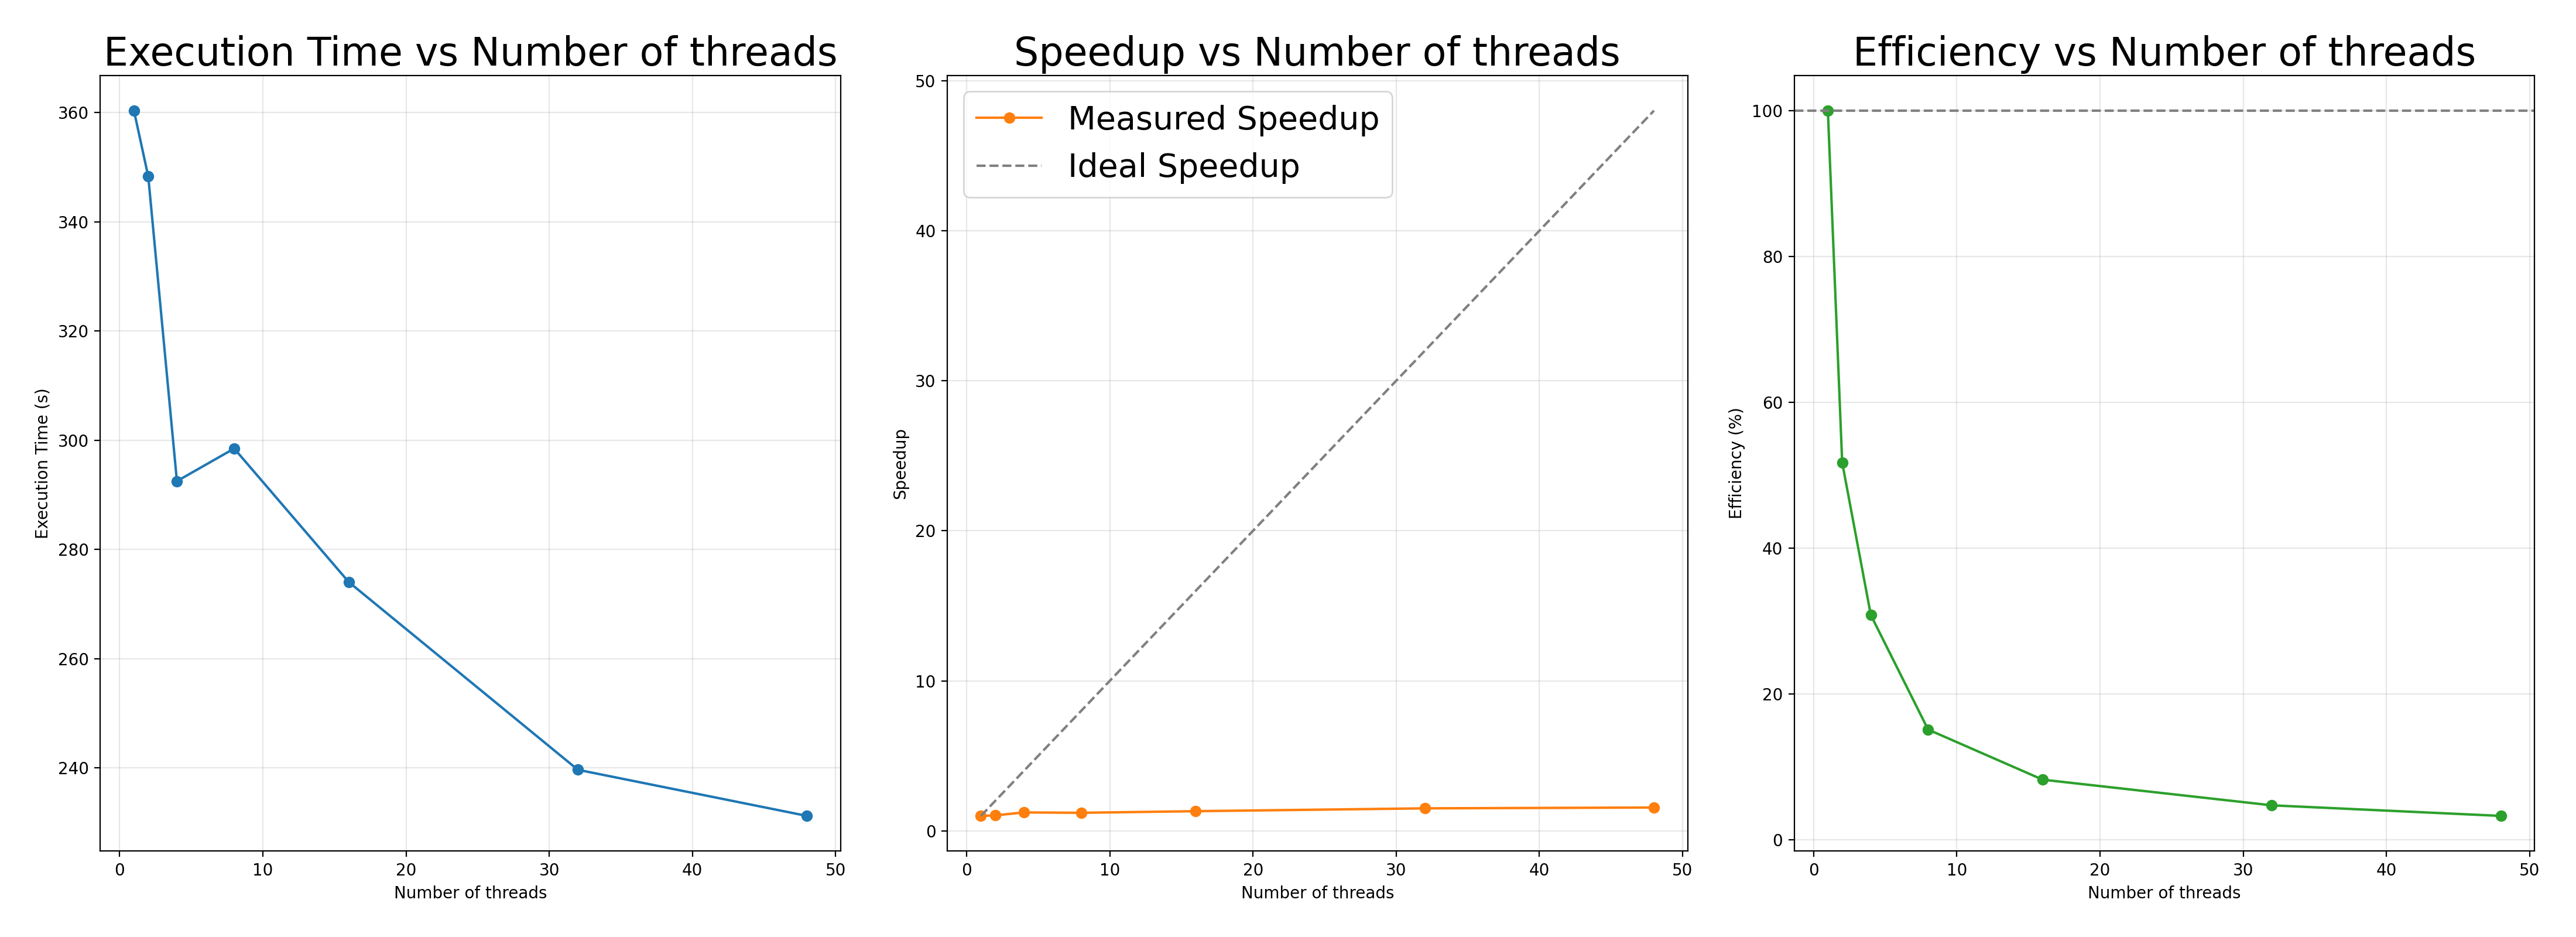
\includegraphics[width=1.0\linewidth]{scaling_plot.png}
\caption{Execution time, speedup, and parallel efficiency as a function of the number of OpenMP threads ($M=2000$, $N=3840$).}
\label{fig:part1-speedup}
\end{figure}

\begin{figure}[h]
\centering
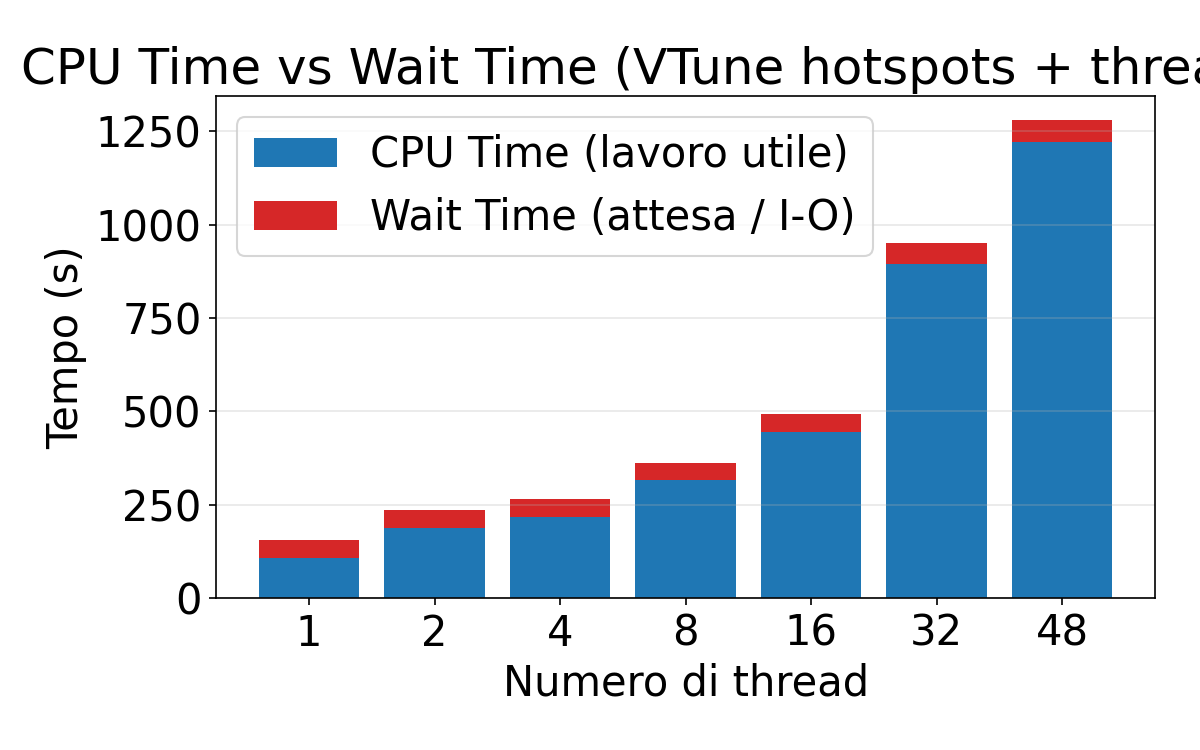
\includegraphics[width=\linewidth]{compute_vs_io_plot.png}
\caption{CPU time (useful computation) vs.\ Wait time (I/O and synchronization) across thread counts, from VTune Hotspots and Threading collections.}
\label{fig:part1-io}
\end{figure}

% =====================================================================
% part2_mpi.tex -- PARTE 2: Estensione multi-simulazione con MPI
% Membro responsabile: ___________________
% Puoi modificare liberamente da qui in poi, non toccare gli altri file.
% =====================================================================
\section{Part 2 -- Multi-Simulation Extension with MPI}
\label{sec:mpi}

\subsection{Problem Description}
The second part of the project extends the OpenMP simulator of Section~\ref{sec:openmp} to
the distributed-memory setting using MPI, with the goal of executing \emph{three independent
simulations simultaneously} on an HPC cluster. Each simulation continues to exploit
intra-node, shared-memory parallelism through OpenMP, resulting in a hybrid MPI+OpenMP
implementation. The three simulations differ in their initial conditions:

\begin{enumerate}[label=(\roman*)]
    \item \textbf{Simulation 1}: identical to the base case of Part~1, with a single impulse
    source at $(i_0,j_0)$ and $t=0$.
    \item \textbf{Simulation 2}: two independent wave sources, located at two distinct points
    of the plane, sharing the same damping $\gamma$ and propagation speed $c$, both activated
    at $t=0$. This configuration is designed to highlight wave interference patterns arising
    from the superposition of the two wavefronts.
    \item \textbf{Simulation 3}: identical to Simulation 2, but the second source is activated
    at a later time $t = t_{\text{start}} > 0$, producing an asymmetric interference pattern.
\end{enumerate}

\subsection{Parallelization Strategy}
The three simulations are mapped onto separate MPI processes (or groups of processes),
allowing them to run concurrently and independently, since there is no data dependency between
them. Each MPI process executes its own instance of the OpenMP-parallelized time-stepping loop
described in Section~\ref{sec:openmp}, writing its output frames to a dedicated folder
(\texttt{sim1}, \texttt{sim2}, \texttt{sim3} respectively). This two-level parallelization
scheme -- MPI across simulations and OpenMP within each simulation -- allows efficient use of
a multi-node cluster where each node hosts one MPI process exploiting all of its available
cores via OpenMP threads.

% TODO (optional): describe communication pattern (if any communication between
% processes is needed, e.g., for synchronized output or load balancing), and how
% the two interfering sources are summed/composed onto the shared grid in
% Simulations 2 and 3.

\subsection{Results}
\textit{[Insert here: simulation parameters for the three runs (Table~\ref{tab:part2-params}),
example frames illustrating single-source propagation and the interference patterns of
Simulations 2 and 3 (Figure~\ref{fig:part2-frames}), and the measured execution time/scalability
of the hybrid MPI+OpenMP implementation as a function of the number of MPI processes and OpenMP
threads.]}

\begin{table}[h]
\centering
\caption{Simulation parameters -- Part 2.}
\label{tab:part2-params}
\begin{tabular}{lccc}
\toprule
Parameter & Sim. 1 & Sim. 2 & Sim. 3 \\
\midrule
$\gamma$               & \textit{TBD} & \textit{TBD} & \textit{TBD} \\
$c$                    & \textit{TBD} & \textit{TBD} & \textit{TBD} \\
Source(s) position     & \textit{TBD} & \textit{TBD} & \textit{TBD} \\
$t_{\text{start}}$ (2nd source) & -- & 0 & \textit{TBD} \\
\bottomrule
\end{tabular}
\end{table}

\begin{figure}[h]
\centering
% \includegraphics[width=\linewidth]{frames_mpi.png}
\caption{Comparison of single-source propagation and multi-source interference patterns. \textit{[Placeholder -- insert figure]}}
\label{fig:part2-frames}
\end{figure}

\begin{figure}[h]
\centering
% \includegraphics[width=\linewidth]{scaling_mpi.png}
\caption{Execution time and scalability of the hybrid MPI+OpenMP implementation. \textit{[Placeholder -- insert figure]}}
\label{fig:part2-scaling}
\end{figure}

\section{Part 3 -- GPU-Accelerated Frame Colorization with CUDA}
\label{sec:cuda}

\subsection{Problem Description}
\label{sec:cuda-problem}

In the first two parts of the project the simulator advances the damped wave and
saves every time step as a grayscale image, where the pixel intensity encodes the
wave height: bright where the wave is high, dark where it is low, mid-gray where
the surface is at rest. The third part does not change the physics at all. Its
only goal is to make the output easier to read by turning each grayscale frame
into a \emph{color} image, so that crests, troughs and calm regions become
immediately distinguishable, and to perform this recoloring on the GPU using
CUDA.

The requirements set by the assignment are: the maxima and minima of the wave
must stand out in bright colors, the rising and falling fronts must use
\emph{different} colors, the calm regions (values close to zero) must be rendered
in a clear color, namely white, and the transition between these must be smooth.
A key point is that the simulation is untouched: the wave keeps evolving on the
original grayscale matrix exactly as before, and the GPU only produces a colored
copy for output. Each colored frame is written to disk as
\texttt{frame\_<xxxxx>.ppm} in the P3 (ASCII) PPM format, the color counterpart
of the grayscale PGM format used previously.

Throughout this section, $M$ denotes the side of the square simulation grid, so
the domain is an $M\times M$ matrix of pixels (for example $M=512$ means a
$512\times512$ image), and $N$ denotes the number of time steps, i.e. the number
of frames produced.

\subsection{Why the GPU}
\label{sec:cuda-why}

Coloring an image means, for each pixel, reading its grayscale value and
computing three numbers (its red, green and blue components). The crucial
observation is that the color of a pixel depends only on that pixel: it does not
need to look at its neighbors. Every pixel can therefore be colored completely
independently of the others. In parallel-computing terms this is an
\emph{embarrassingly parallel} problem, there are no dependencies and no
communication between the units of work, and it is exactly the kind of workload
a GPU is designed for.

A CPU has a few powerful cores; a GPU has thousands of simple cores that all
execute the same instruction on different data at the same time. For a task made
of hundreds of thousands of identical, independent operations (one per pixel),
the GPU is the natural choice. This also changes how the code is written compared
to the OpenMP version of Section~\ref{sec:openmp}. In OpenMP we write the two
nested loops over the pixels and a \texttt{\#pragma} distributes the iterations
across the cores. In CUDA the loops disappear: we write the work of a
\emph{single} pixel and launch it on a grid of threads, one thread per pixel.
Each thread figures out on its own which pixel it is responsible for.

There is a cost specific to the GPU that OpenMP does not have. The CPU and the
GPU have separate memories: the GPU cannot directly read the CPU's RAM. Before
coloring, the grayscale matrix must be copied from CPU memory to GPU memory
(host-to-device, H2D); after coloring, the RGB result must be copied back
(device-to-host, D2H) so the CPU can write it to disk. Each frame is therefore a
three-stage pipeline -- copy in, color, copy out -- and, as the results below
show, moving the data turns out to cost far more than coloring it.

\subsection{The Color Transfer Function}
\label{sec:cuda-colorfun}

The assignment asks for ``a suitable mathematical transformation function'' that
maps a grayscale value to an RGB triplet. We build it in three steps.

\paragraph{Step 1: from grayscale to a signed deviation.}
The grayscale value $g\in[0,255]$ already encodes where the wave is: after the
normalization of Part~1, $g=127$ is the rest level, $g=255$ a maximum crest and
$g=0$ a minimum trough. Working with a value centered on $127$ is awkward, so we
first re-center it around zero:
\begin{equation}
    d = \frac{g - 127.5}{127.5} \in [-1,\,+1].
    \label{eq:cuda-d}
\end{equation}
Now $d=0$ is calm water, $d=+1$ a maximum crest, $d=-1$ a minimum trough. The
single number $d$ carries both the \emph{sign} (crest vs.\ trough) and the
\emph{magnitude} (how far from calm) of the displacement.

\paragraph{Step 2: the sign chooses the color.}
We use a three-anchor scale: calm ($d=0$) is white, a crest ($d=+1$) is pure red,
a trough ($d=-1$) is pure blue. The sign of $d$ selects which half of the scale
to use, positive goes toward red, negative toward blue, so rising and falling
fronts automatically receive different colors, as required. A neutral color in
the middle with two opposite bright colors at the ends is known as a
\emph{diverging} color map, and it is the appropriate choice whenever the data
has a meaningful zero with symmetric positive and negative values, as ours
does.\footnote{See K.\ Moreland, ``Diverging Color Maps for Scientific
Visualization'', ISVC 2009.}

\paragraph{Step 3: a non-linear correction so the wave stays visible.}
A direct linear use of $d$ fails here, for a physical reason. The wave is
\emph{damped}: its amplitude decays enormously over time, in our runs, by about
three orders of magnitude, from roughly $30$ at the first frame to about $0.03$
near the end. Since the color scale is fixed on the initial amplitude, after a
few dozen frames the wave occupies less than $1\%$ of the scale: every value maps
to a gray extremely close to $127$, $d$ becomes tiny, and the whole frame turns
almost pure white. The ripples are still in the data, but they are invisible.

To fix this we must amplify the small values without disturbing the ordering
(the largest displacements must remain the brightest). This is achieved by
raising $|d|$ to a power smaller than one:
\begin{equation}
    d' = \operatorname{sign}(d)\,|d|^{\,\gamma_c},
    \qquad \gamma_c = 0.30.
    \label{eq:cuda-gamma}
\end{equation}
A concrete example makes the effect clear. A weak late-time front with $d=0.008$
becomes $0.008^{0.3}\approx 0.24$, i.e.\ it goes from ``almost white'' to a
clearly visible color; a strong early front with $d=0.8$ becomes
$0.8^{0.3}\approx 0.94$, essentially unchanged. The power law compresses the
range: it lifts the small values a lot and the large values very little. Because
it is a monotonic function, it never reorders the values, what was higher stays
higher. The $\operatorname{sign}(d)$ factor simply restores the sign after the
exponentiation, which acts on the magnitude $|d|$. The exponent $\gamma_c$ is a
single contrast knob: $\gamma_c=1$ gives back the useless linear map, and smaller
values increase the contrast. This is the same power-law correction used for
\emph{gamma} in digital imaging, where it is applied because human brightness
perception is itself non-linear and more sensitive to differences among dark
tones than bright ones.\footnote{See C.\ Poynton, ``Digital Video and HD:
Algorithms and Interfaces'', 2003; the underlying psychophysical power law is due
to S.\ S.\ Stevens (1957).}

\paragraph{Final RGB.}
Given the corrected value $d'$, the three color channels are obtained by
interpolating between white and the appropriate saturated extreme:
\begin{equation}
    (R,G,B) =
    \begin{cases}
      \bigl(255,\; 255(1-d'),\; 255(1-d')\bigr), & d' \ge 0,\\[4pt]
      \bigl(255(1+d'),\; 255(1+d'),\; 255\bigr), & d' < 0.
    \end{cases}
    \label{eq:cuda-rgb}
\end{equation}
For $d'\ge 0$ the red channel stays at $255$ while green and blue fall from $255$
to $0$, so the color goes smoothly from white to red; for $d'<0$ the roles are
mirrored and the color goes from white to blue. The interpolation gives the
smooth fade required by the assignment, with no hard banding at the midpoint.

\subsection{Kernel Implementation}
\label{sec:cuda-kernel}

The transfer function above is evaluated by a CUDA \emph{kernel}, a function that
runs on the GPU and is launched from the CPU. It is launched with one thread per
pixel of the $M\times M$ grid, with the threads grouped into $16\times16$ blocks.
Instead of looping over the pixels, each thread computes the coordinates $(i,j)$
of ``its'' pixel from its position in the grid of blocks, reads the corresponding
grayscale value, applies Equations~\eqref{eq:cuda-d}--\eqref{eq:cuda-rgb}, and
writes the resulting triplet into an interleaved RGB buffer (the three channels
of a pixel stored consecutively). Because the grid is rounded up to a whole
number of blocks, a few threads may fall outside the image; a simple bounds check
makes them do nothing. Since each pixel is independent, the kernel needs no
synchronization between threads.

Only the coloring runs on the device: as required, the simulation itself keeps
running on the host on the original grayscale matrix. The device buffers are
allocated once and reused for every frame, rather than allocated and freed each
time, because GPU allocation is a relatively expensive operation.

\subsection{Results}
\label{sec:cuda-results}

\subsubsection{Visual Correctness}

Figure~\ref{fig:cuda-frames} shows representative colored frames at different
stages of the simulation. The result matches what the assignment asks for: the
calm background is white, the wavefront appears as a set of concentric colored
rings, crests and troughs are shown in saturated red and blue, and the damping is
visible as the colors fade back toward white over time. The circular symmetry of
the fronts, preserved by the 9-point isotropic Laplacian of
Section~\ref{sec:openmp}, becomes obvious once the field is colored.

% --------- FIGURA FRAME COLORATI: scommenta quando hai le immagini ---------
\begin{figure}[t]
    \centering
    \begin{subfigure}{0.32\linewidth}
        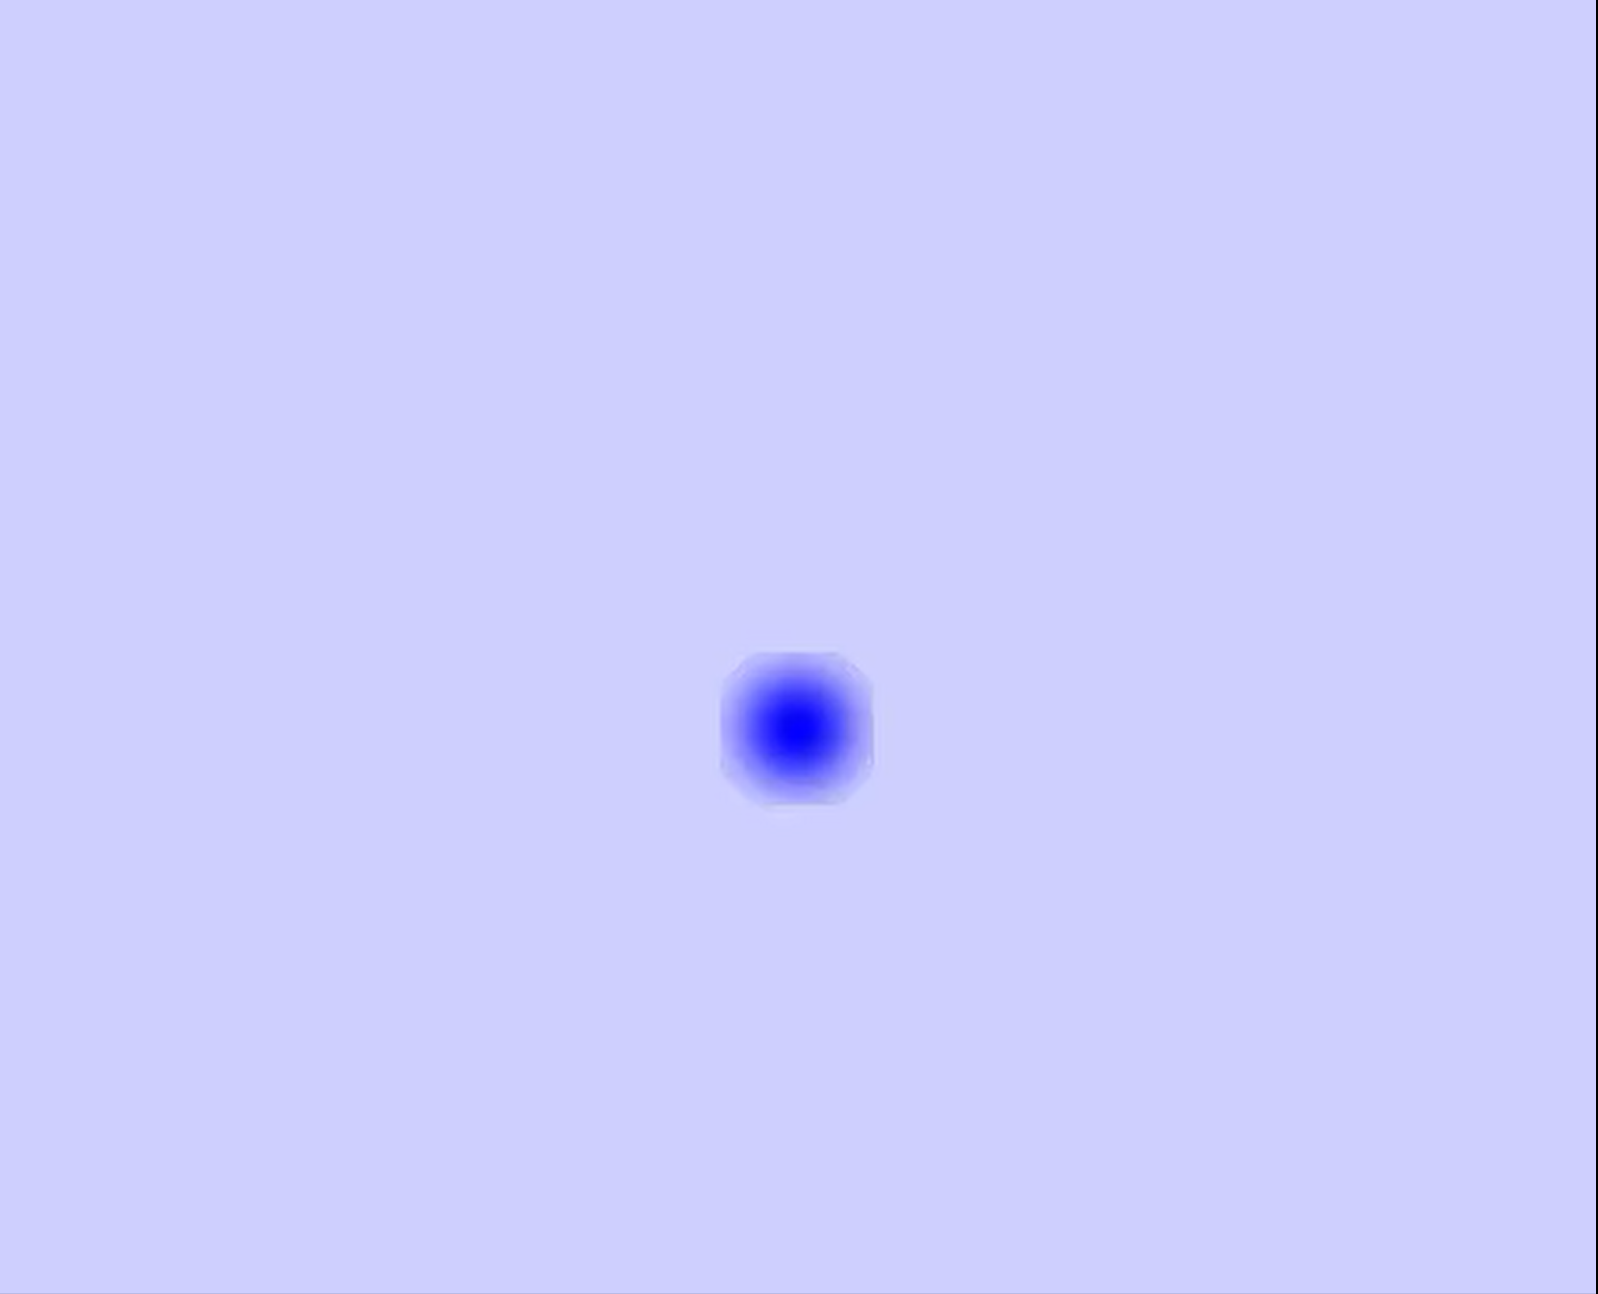
\includegraphics[width=\linewidth]{ph1.png}
        \caption{$t = 0$}
    \end{subfigure}\hfill
    \begin{subfigure}{0.32\linewidth}
        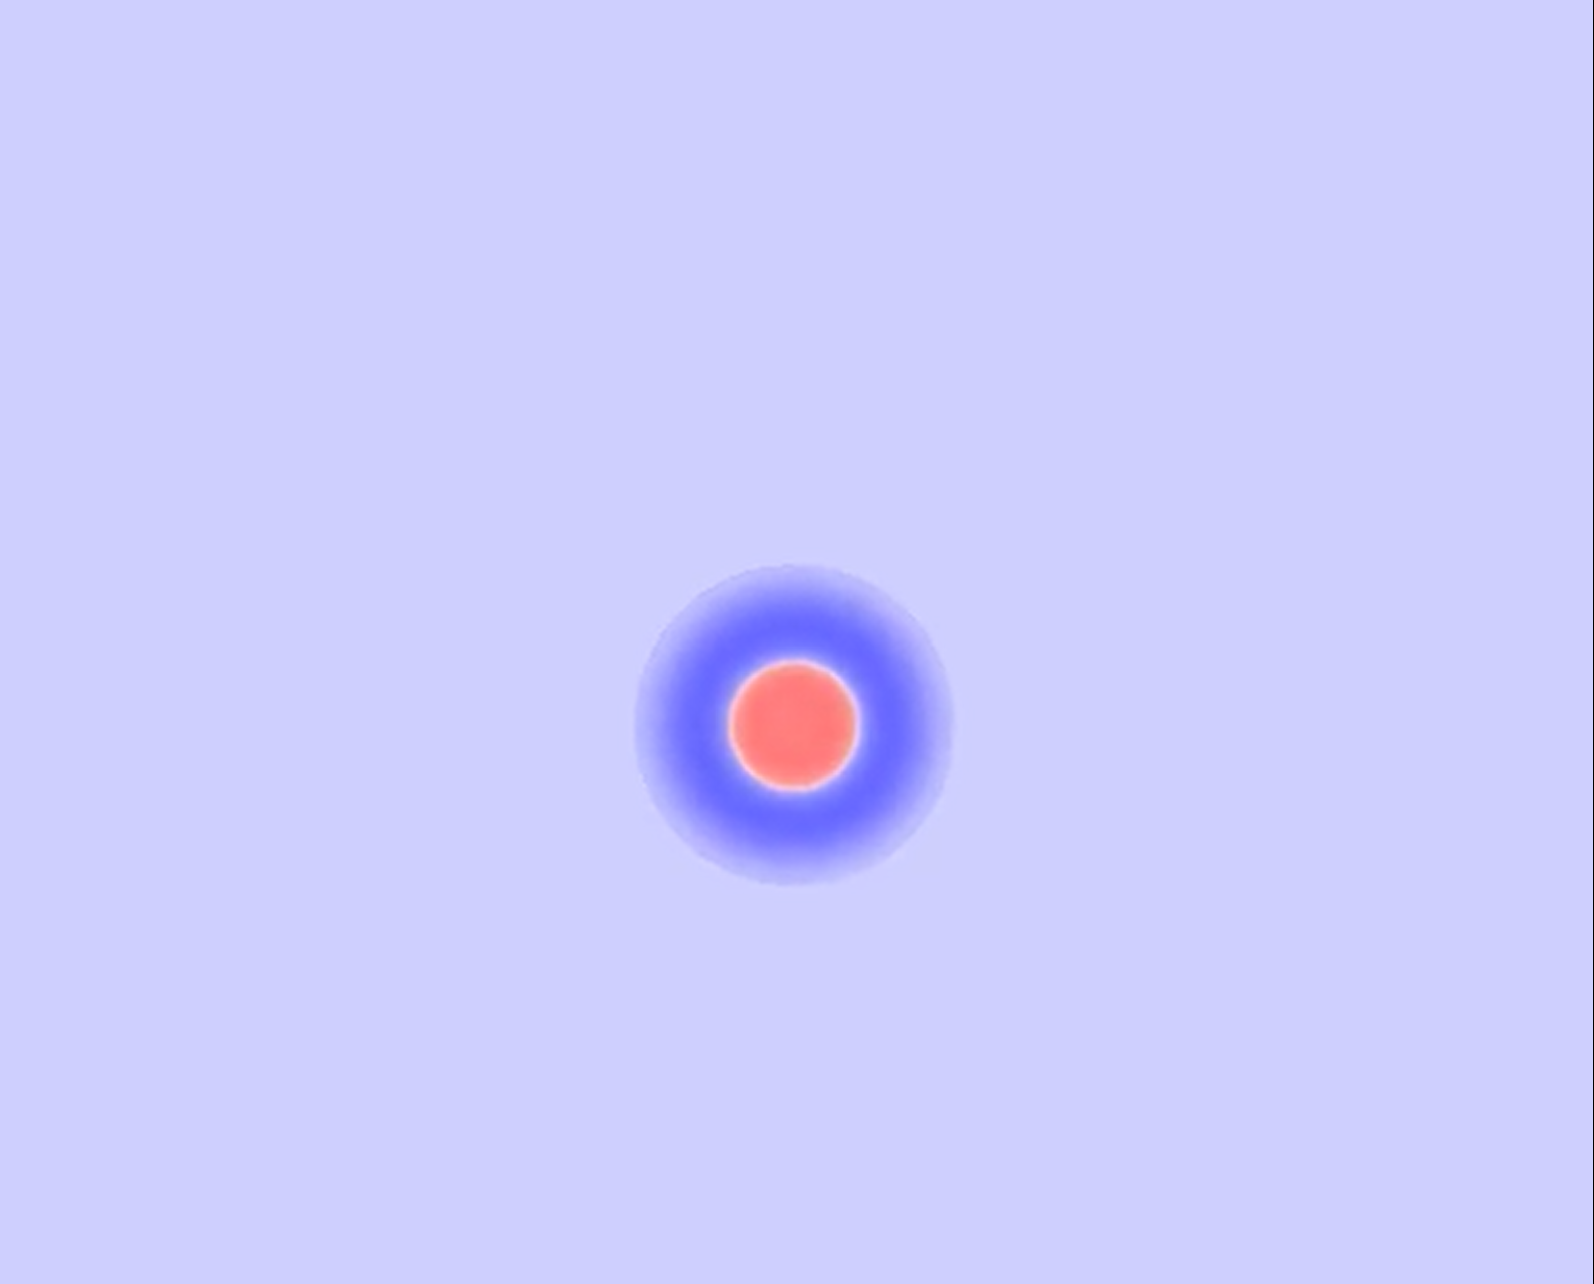
\includegraphics[width=\linewidth]{ph2.png}
        \caption{$t > 0$}
    \end{subfigure}\hfill
    \begin{subfigure}{0.32\linewidth}
        
\includegraphics[width=\linewidth]{ph3.png}
        \caption{$t > N/2$}
    \end{subfigure}
    \caption{Example frames of the colorized wave simulation at different time
    steps. Troughs are rendered in blue, crests in red, and calm regions in
    white; the progressive fading of the colors reflects the damping of the wave
    amplitude.}
    \label{fig:cuda-frames}
\end{figure}

\subsubsection{How the Timings Were Measured}

As explained in Section~\ref{sec:cuda-why}, each frame goes through three GPU
stages: the H2D copy of the grayscale matrix, the kernel that colors it, and the
D2H copy of the RGB result. We measure these three stages separately using CUDA
\emph{events}, which record time on the GPU itself;

Two precautions make the numbers meaningful. First, a \emph{warm-up}: the very
first kernel launch of a program also pays a one-time cost for setting up the
CUDA context and loading the code onto the GPU. If this is charged to the first
measured frame it completely distorts the average, we observed an apparent
$1.22$~ms per frame over $30$ frames versus $0.0096$~ms per frame over $200$, for
the same kernel. We therefore run one untimed ``warm-up'' launch before starting
the measurements, so the reported figures reflect the true steady-state cost.
Second, the writing of the PPM file is disk I/O, not GPU work, so it is
deliberately kept out of the GPU timings; it nevertheless remains the single most
expensive stage of the whole program.

\subsubsection{The Kernel Is Cheap; the Transfers Are Not}

With this methodology the kernel itself turns out to be extremely fast. At
$M=512$ it colors more than $260\,000$ pixels in about $0.01$~ms, and even at
$M=2048$ (over four million pixels) it stays around $0.06$~ms per frame. The
consequence is striking: on the GPU side, the runtime is almost entirely spent on
the two data transfers across the PCIe bus, which together account for roughly
$85$--$90\%$ of the device-side time, while the actual computation is a few
percent.

So, for this problem the arithmetic is cheap and the real cost lies in moving data, here across the PCIe bus between CPU and GPU and, in absolute terms even more, in writing the frames to disk. Recognizing these transfers as the bottleneck is what motivates the optimization in the next subsection.

\subsubsection{An Optimization Beyond the Requirements: Pinned Host Memory}
\label{sec:cuda-pinned}

Optimizing the transfers is not part of the assignment, but since they dominate
the GPU time we investigated the standard technique for this situation:
\emph{pinned} host memory. Ordinary host buffers, allocated with \texttt{malloc},
are \emph{pageable}, meaning the operating system is free to move those memory
pages around (or swap them to disk). Because the GPU's DMA engine copies from
fixed physical addresses, it cannot read pageable memory directly: the driver
must first copy the data into a temporary locked buffer and only then transfer
it, so every byte is copied twice. Allocating the buffers with
\texttt{cudaHostAlloc} instead makes them \emph{pinned} (page-locked): the memory
is nailed to a fixed physical location, the DMA engine reads it directly, and the
intermediate copy disappears.

This comparison is a controlled experiment. Both executables are built from
exactly the same source files; the only difference is a single compile flag
(\texttt{-DUSE\_PINNED\_MEMORY}) that switches the allocation from \texttt{malloc}
to \texttt{cudaHostAlloc}. Any measured difference can therefore be attributed to
the memory type alone, and not to some other change in the code.

Figure~\ref{fig:cuda-pinned} and Table~\ref{tab:cuda-pinned} report a sweep over
the grid size $M$, with each configuration run three times and the median kept
(the node is shared, so repeating guards against the occasional interference from
other jobs). Three things stand out. The transfers become faster, with a peak
speedup of $2.15\times$ at $M=512$. The effective host-to-device bandwidth nearly
doubles, from about $14$~GB/s with pageable memory to about $25$~GB/s with pinned
memory at the larger sizes, the latter close to the practical limit of the PCIe
link. And, as a sanity check, the kernel time is essentially identical in the two
builds ($0.0085$ vs.\ $0.0082$~ms at $M=512$), confirming that pinned memory
affects only the data transfers and not the computation, exactly as expected.

% --------- FIGURA GRAFICI PINNED: scommenta, l'immagine ce l'hai gia' ---------
 \begin{figure}[t]
     \centering
     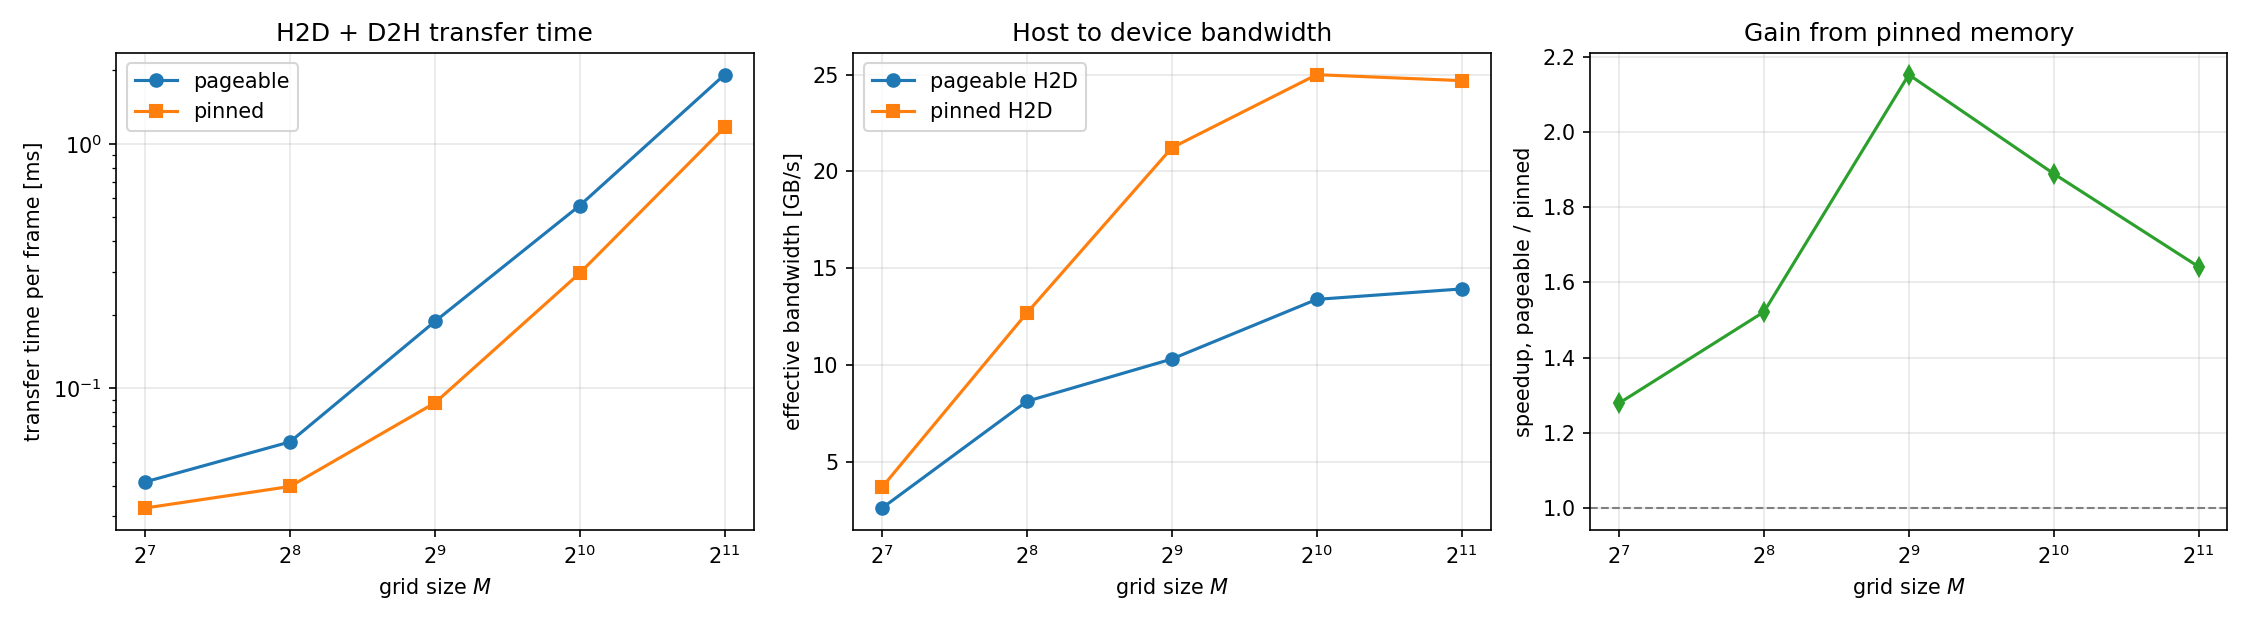
\includegraphics[width=\linewidth]{cuda_pinned_comparison.png}
     \caption{Pageable vs.\ pinned host memory as a function of the grid size $M$.
     Left: combined H2D$+$D2H transfer time per frame. Center: effective
     host-to-device bandwidth. Right: transfer-time speedup of pinned over
     pageable. Medians over three repetitions.}
     \label{fig:cuda-pinned}
 \end{figure}

The speedup is not constant across sizes: it rises up to $M=512$ and then eases
back to $1.6$--$1.9\times$ at the largest grids. The reason is intuitive. At
small sizes the transfer is dominated by a fixed per-call overhead that pinning
does not remove, so the benefit is modest. At intermediate sizes the raw
bandwidth becomes the limiting factor and pinning helps the most. At the largest
sizes the pinned bandwidth saturates near the PCIe ceiling while the pageable
path still gains a little from internal buffering, so the ratio settles. There is
thus a ``sweet spot'' around $M=512$ where pinned memory is most effective.
\begin{table}[t]
    \centering
    \caption{Transfer time per frame (H2D$+$D2H) and effective host-to-device
    bandwidth, pageable vs.\ pinned host memory. Medians over three repetitions.}
    \label{tab:cuda-pinned}
    \setlength{\tabcolsep}{4pt}
    \small
    \begin{tabular}{rrrrr}
        \toprule
        $M$ & pag.\ [ms] & pin.\ [ms] & speedup & BW pin.\ [GB/s] \\
        \midrule
        128  & 0.0412 & 0.0336 & $1.23\times$ & 3.72 \\
        256  & 0.0605 & 0.0398 & $1.52\times$ & 12.71 \\
        512  & 0.1878 & 0.0873 & $2.15\times$ & 21.22 \\
        1024 & 0.5511 & 0.2961 & $1.86\times$ & 24.99 \\
        2048 & 1.9168 & 1.1678 & $1.64\times$ & 24.68 \\
        \bottomrule
    \end{tabular}
\end{table}

% =====================================================================
\section{Conclusions}
% =====================================================================
This report described the incremental development of a damped wave
equation simulator across
three parallel computing paradigms. The OpenMP implementation
established a correct and
efficient shared-memory baseline; the MPI extension enabled the
concurrent execution of
multiple independent simulations, including the study of wave
interference phenomena, in a
hybrid MPI+OpenMP fashion suitable for multi-node HPC clusters; and
the CUDA stage demonstrated
how GPU acceleration can be effectively applied to a massively
data-parallel post-processing
task, improving the visual interpretability of the simulation results
without affecting the
underlying numerical computation. 

% =====================================================================
% \section*{References}
% Aggiungere la bibliografia qui se richiesta dal corso, ad es. con
% \texttt{thebibliography} oppure un file \texttt{.bib} con
% \texttt{natbib}/\texttt{biblatex}.
% =====================================================================

\end{document}
